
\subsection{Additional Results of Logistic Regression Experiments}


\begin{figure}[H]
  \centering
  \subfloat[Pima]{
    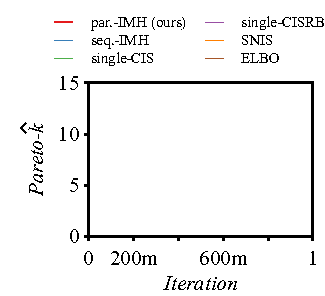
\includegraphics[scale=0.80]{figures/pima_01.pdf}
  }
  \subfloat[Heart]{
    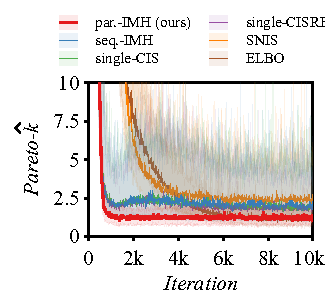
\includegraphics[scale=0.80]{figures/heart_01.pdf}
  }
  \caption{Pareto-\(\widehat{k}\) results of logistic regression problems.
    The solid lines are the median of 100 repetitions while the colored regions are the 80\% empirical percentiles.
  }
\end{figure}

%%% Local Variables:
%%% TeX-master: "master"
%%% End:
